% IS-LM diagram
% Author: Tarik Ocaktan
% Original code taken from: http://www.texample.net/tikz/examples/is-lm-diagram/ 
\documentclass{minimal}
\usepackage{tikz}
\usepackage{verbatim}

\begin{comment}
:Title: Demand-supply diagram
:Tags: Diagrams, Plots, Coord. calculations

This figure shows a shift demand and supply

.. _Supply-Demand curve: https://en.wikipedia.org/wiki/Supply_and_demand

:Author: Tarik Ocaktan (February 2020)

LM-->AS 
IS-->AD

\end{comment}



\usetikzlibrary{arrows,calc}
\usepackage{relsize}
\newcommand\AS{\ensuremath{\mathit{AS}}}
\newcommand\AD{\ensuremath{\mathit{AD}}}
\begin{document}

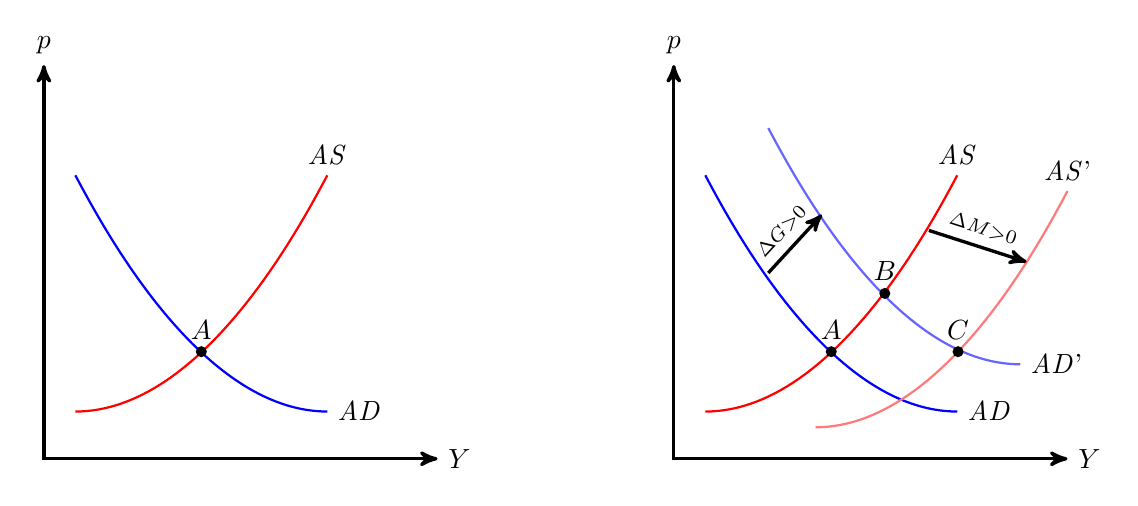
\begin{tikzpicture}[
        scale=2,
        AD/.style={blue, thick},
        AS/.style={red, thick},
        axis/.style={very thick, ->, >=stealth', line join=miter},
        important line/.style={thick}, dashed line/.style={dashed, thin},
        every node/.style={color=black},
        dot/.style={circle,fill=black,minimum size=4pt,inner sep=0pt,
            outer sep=-1pt},
    ]
    % axis
    \draw[axis,<->] (2.5,0) node(xline)[right] {$Y$} -|
                    (0,2.5) node(yline)[above] {$p$};
    % AD-AS diagram
    \draw[AS] (0.2,0.3) coordinate (AS_1) parabola (1.8,1.8)
        coordinate (AS_2) node[above] {\AS};
    \draw[AD] (0.2,1.8) coordinate (AD_1) parabola[bend at end]
         (1.8,.3) coordinate (AD_2) node[right] {\AD};

    \node[dot,label=above:$A$] at (1,.68) (int1) {};
        

    \begin{scope}[xshift=4cm]
     \draw[axis,<->] (2.5,0) node(xline)[right] {$Y$} -|
                    (0,2.5) node(yline)[above] {$p$};
    % AD-AS diagram
    \draw[AS] (0.2,0.3) coordinate (AS_1) parabola (1.8,1.8)
        coordinate (AS_2) node[above] {\AS};
    \draw[AD] (0.2,1.8) coordinate (AD_1) parabola[bend at end]
         (1.8,.3) coordinate (AD_2) node[right] {\AD};

    %Intersection is calculated "manually" since Tikz does not offer
    %intersection calculation for parabolas
    \node[dot,label=above:$A$] at (1,.68) (int1) {};
    %shifted AD-AS diagram
    \draw[xshift=.7cm, AS, red!52] (0.2,0.2) parabola (1.8,1.7)
        node[above] {\AS'};
    \draw[xshift=.4cm, yshift=.3cm, AD, blue!60] (0.2,1.8)
        parabola[bend at end] (1.8,.3)
        node[right] {\AD'};
    %Intersection of shifted AD-AS
    \path[xshift=.36cm, yshift=.35cm] (.98,.7)
        node[dot,label=above:{$B$}] (int2) {};
    \path[xshift=.805cm] (1,.68) node[dot,label=above:$C$] (int3) {};
    %arrows between intersections
    \draw[->, very thick, black, >=stealth']
        ($(int1)+1/2*(-.80,1)$) -- ($(int2)+1/2*(-.8,1)$)
        node[sloped, above, midway] {$\mathsmaller{\Delta G > 0}$};
    \draw[->, very thick, black, >=stealth']
        ($(int2)+2*(.14,.2)$) -- ($(int2)!.2cm!270:(int2)+(.9,0)$)
        node[sloped,above, midway] {$\mathsmaller{\Delta M>0}$};


    \end{scope}




\end{tikzpicture}
\end{document}
%%% Local Variables:
%%% mode: latex
%%% TeX-master: 
%%% End:
